\chapter{Methodik}
\label{chap:methodik}

Für die Segmentierung der Marsoberfläche wird der Ansatz von Kanezaki \etal \cite{kanezaki_18} aus Unterabschnit~\ref{ssec:kanezaki} abgewandelt. Das Ziel besteht daraus, eine Eingabebilddatei durch neuronale Netze zu segmentieren, allerdings ohne vorhandene Ground Truth.

Zur Modifikation des genannten Algorithmus existieren viele unterschiedliche Möglichkeiten, einzelne Elemente zu ersetzen, welche in den folgenden Abschnitten beschrieben werden.

\section{Initialisierung}
\label{sec:initialisierung}

Die wohl wichtigste Veränderung des ursprünglichen Algorithmus besteht aus der Modifizierung des Initialisierungsalgorithmus.

Der von Kanezaki \etal genutzte SLIC-Algorithmus eignet sich zwar gut für die meisten mehrfarbigen Fotografien, da die Aufnahmen der Marsoberfläche allerdings nur in Graustufen vorhanden sind, würden so hier keine guten Ergebnisse produziert werden.

\begin{figure}[h!]
	\centering
	\begin{subfigure}[t]{0.32\textwidth}
		\centering
		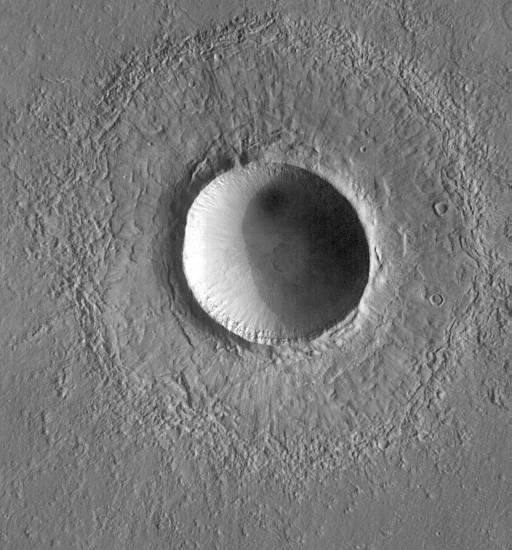
\includegraphics[width=\textwidth,keepaspectratio]{images/Gre13_01.jpg}
		\captionsetup{format=plain,width=0.85\textwidth}
		\caption{Eingabebild, aus \cite[Kap.~7]{greeley_13}}
		\label{fig:slic_vs_tsugf_in}
	\end{subfigure}
	\hfill
	\begin{subfigure}[t]{0.32\textwidth}
		\centering
		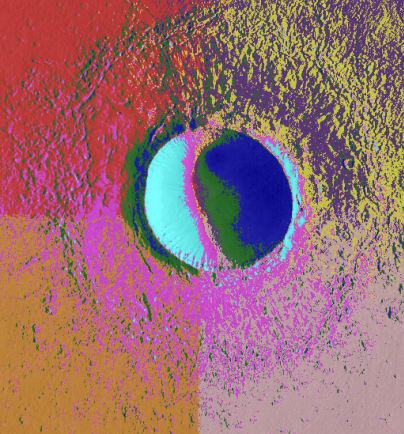
\includegraphics[width=\textwidth,keepaspectratio]{images/gen/GEN_slic_vs_tsugf_01.png}
		\captionsetup{format=plain,width=0.85\textwidth}
		\caption{Ergebnis des SLIC-Algorithmus angewandt auf die Eingabedatei}
		\label{fig:slic_vs_tsugf_slic}
	\end{subfigure}
	\hfill
	\begin{subfigure}[t]{0.32\textwidth}
		\centering
		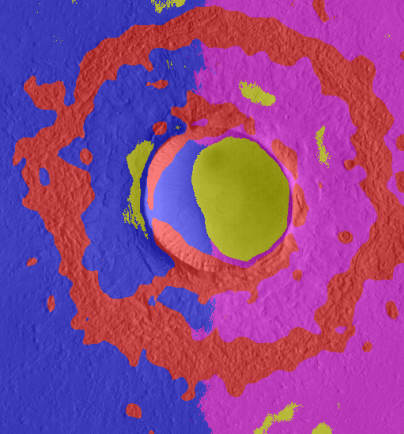
\includegraphics[width=\textwidth,keepaspectratio]{images/gen/GEN_slic_vs_tsugf_02.png}
		\captionsetup{format=plain,width=0.85\textwidth}
		\caption{Ergebnis des texturbasierten Clusterings der Eingabedatei}
		\label{fig:slic_vs_tsugf_tsugf}
	\end{subfigure}
	\caption{Clustering eines Graustufenbildes}
\end{figure}

So ergibt ein Clustering des Kraters aus Unterabschnitt~\ref{ssec:mars_surface} durch den SLIC-Algorithmus \cite{achanta_10} das in \figurename~\ref{fig:slic_vs_tsugf_slic} sichtbare Ergebnis.\footnote{SLIC-Implementierung: \texttt{scikit-image}\\Parameter: \texttt{compactness=5, n\_segments=10, enforce\_connectivity=False}} Dort ist erkennbar, dass der Krater in jeweilige Licht- und Schattenregionen (bedingt durch den Lichteinfall im flachen Winkel) unterteilt wird. Außerdem wird die raue Struktur ringförmig um den Krater herum schlecht erfasst: An dieser Stelle wird jeder Hügel separat als einerseits helle, andererseits dunkle Stelle markiert. Das Phänomen, dass ein Krater so durch eine starke Differenz an Licht- und Schattenregionen äußert wird sich im Großen und Ganzen zwar in Abschnitt~\ref{sec:craterdetection} zu nutze gemacht, ist hier allerdings ungewollt.

Wenn nun der in Unterabschnitt~\ref{ssec:kanezaki} beschriebene Ansatz verfolgt wird, wird das neuronale Netz daraufhin trainiert, eine Aufnahme anhand ihrer Helligkeitsinformationen hin zu trainieren. Da dies nicht gewollt ist, wird statt einem farb-/helligkeitsbasierten Clusteringalgorithmus wie SLIC ein texturbasiertes Clustering genutzt.

Statt des SLIC-Clusterings wird nun die in Unterabschnitt~\ref{ssec:tsugf} vorgestellte Methode des texturbasierten Clusterings genutzt. Von dieser Stelle an sind --~wenn nicht anders benannt~-- die Gewichtungen der verschiedenen Werte für die Farbwerte, X-/Y-Positionen und Reaktion auf Gaborfilter alle gleich $1$. Diese Parameter werden in Unterabschnitt~\ref{ssec:filterweight} genauer erläutert.

Das Ergebnis eines Clusterings durch die genutzte, texturbasierte Methode\footnote{Kombiniert mit der Filterbank aus \cite{jain_91}} ist in \figurename~\ref{fig:slic_vs_tsugf_tsugf} sichtbar: Man erkennt, dass der \enquote{Ring} um den eigentlichen Einschlagskrater eine eigenständige Textur besitzt, welche unterschiedlich zu dem Rest der Oberfläche ist. Eine ähnliche Oberflächenstruktur ist direkt um den Krater herum vorhanden. Beide Vorkommnisse dieser ähnlichen Struktur werden vom texturbasierten Clustering erfasst, in ein Segment aufgeteilt und (hier durch eine rote Färbung) markiert.

\subsection{Filterbänke}

Nun stellt sich die Frage, welche der vorgestellten Filterbänke sich gut eignet, die Eingabedatei zu clustern. Die größten Unterschiede zwischen den einzelnen Filterbänken besteht daraus, dass einige von ihnen rotationsinvariante Filter enthalten, und einige in mehreren Größen vorhanden sind. Die Größendifferenz lässt sich zwar in der Anwendung des Algorithmus ausgleichen, die Rotationsinvarianz allerdings nicht. In \figurename~\ref{fig:filterbank_comparision} ist die Anwendung der in Unterabschnitt~\ref{ssec:tsugf} vorgestellten Filterbänke auf vier Beispielbilder (\vgl Abschnitt~\ref{ssec:mars_surface}) sichtbar. Jedes Bild wurde in vier Cluster aufgeteilt und alle Optimierungen (\vgl Unterabschnitt~\ref{ssec:tsugf}) des Verfahrens wurde angewandt.

\paragraph{Krater}
Neben dem eigentlichen Krater ist auf dieser Aufnahme der Ring aus gröberem Gestein signifikant. Dieser wird von allen Filterbänken zuverlässig erkannt, wenn auch mit einer unterschiedlichen Dicke: Die LM- und S-Filterbank selektieren dieses Gestein eher großzügig, die MR-Filterbank hingegen zeigt sehr enge Markierungen dieser Region.

Alle Filterbänke formen einen Ring (oder dessen Ansatz) auf dem Kraterrand, die Maximum Response-Filterbank erzeugt zwei konzentrische Ringe

Der Krater selbst wird von den Filterkombinationen nach \cite{jain_91} und der LM-Filterbank leider nur in Hell- und Dunkel-Regionen aufgeteilt, die S-Filterbank zeigt innerhalb des Kraters kein brauchbares Ergebnis. Eine Ausnahme stellt die Maximum-Response-Filterbank dar, welche neben den zwei erwähnten konzentrischen Clustern den Bereich innerhalb des Kraters als ein einziges Cluster erkennt. Die Maximum Response-Bank erzeugt in diesem Bereich das Ergebnis, welches sich wohl als bestes zur Weiterverarbeitung eignet.

\paragraph{Vulkan}
Der Vulkanberg wird leider von keiner Filterbank optimal erkannt. Der äußere Rand wird nur von der S-Filterbank als ein Cluster erkannt, dies allerdings nicht sehr genau. Der rauere Bereich der Oberfläche, was kleinere Krater miteinbeschließt, wird vom MR-Filter am ehesten und genausten erkannt (in violett markiert), auf dem zweiten Platz folgt die Filterbank nach \cite{jain_91}, welche zwar alle Krater in ein Cluster fügt (violett), allerdings eher gröber.

Die Vulkanmitte wird von keiner Filterbank erkannt, nur bei der MR-Bank lässt sich eine ringförmige, rauere Stelle um den Krater herum erahnen. Außerdem ist interessant, dass der LM-Filter die Bergspitzen in vom Umfeld getrennte Cluster einteilt (blau und violett). Somit scheint es, als ließe sich diese Aufnahme über keine Filterbank gut clustern, am ehesten eignet sich allerdings erneut die MR-Bank.

\paragraph{Vulkan mit strahlenförmigen Merkmalen}

Das Ziel bei der Nutzung dieser Marsaufnahme zur Analyse besteht daraus zu analysieren, mit welcher Filterbank die konzentrischen Strahlen am genauesten erkannt werden. Des Weiteren existieren auf der Aufnahme noch Krater, welche es separat zu clustern gilt.

Die Filterbank nach \cite{jain_91} erkennt die gröberen Strukturen (Strahlen und Krater), fügt diese allerdings in dasselbe Cluster ein (gelb und rot).

Die LM-Filterbank scheint kein brauchbares Ergebnis zu produzieren, sie erkennt im Allgemeinen nur einige der Krater (gelb) separat von deren Umfeld, die Strahlen sind nicht geeignet geclustert worden.

Die Schmid-Filterbank clustert einen Großteil der Strahle gemeinsam in ein Cluster (rot). Die Krater hingegen sind nicht fest einer Clusterart zugewiesen.

Wie in den vorherigen Test ist das Ergebnis der MR-Filterbank schon fast zu genau, die Cluster sind sehr fein gehalten. Im Gegensatz zu den Alternativen, werden hier die Krater relativ zuverlässig in gelbe Cluster eingeordnet, die Strahlen sind leider zu fein, als das sie getrennt erkennbar sind. Dieses Phänomen könnte sich allerdings in der praktischen Anwendung zunutze gemacht werden, da dafür eine zu feine Initialisierung notwendig ist.

\paragraph{Gletscher}

Der Gletscher ist subjektiv betrachtet das schwierigste der hier vorgestellten Probleme, da er an vielen seiner Ränder keine feste Grenze zu benachbarten Regionen zeigt, nur links auf der Aufnahme ist er durch eine Hügelreihe strikt begrenzt. Diese Grenze wird von allen Filterbänken in ein getrenntes Cluster unterteilt,mit Ausnahme der Filterbank nach \cite{jain_91}: Diese produziert kein geeignetes Ergebnis, nur die stärker erkennbaren \enquote{Streifen} werden gut erkannt (blau). Die LM-Filterbank erkennt zwar die Abgrenzung auf der linken Seite, allerdings keine anderen Regionen korrekt. Sie liefert bei diesem Bild das wohl schlechteste Ergebnis. Die Maximum-Response Methode und die Filterbank nach \cite{leung_01} liefern zwar etwas bessere Ergebnisse, diese sind allerdings nicht gut. Die MR-Bank erzeugt erneut sehr feine Cluster.

\paragraph{}
Zusammengefasst erzeugt aus dieser Auswahl an Filterbänden die Maximum Response-Methode von \cite{visgeo} das wohl am ehesten geeignete Ergebnis zur Weiterverarbeitung. Auf zweitem Platz folgt die Schmid-Filterbank.

\begin{figure}[h!]
\setlength\tabcolsep{1pt}
\def\arraystretch{0.5}
\begin{tabular}{p{0.2\textwidth}p{0.2\textwidth}p{0.2\textwidth}p{0.2\textwidth}p{0.2\textwidth}}
	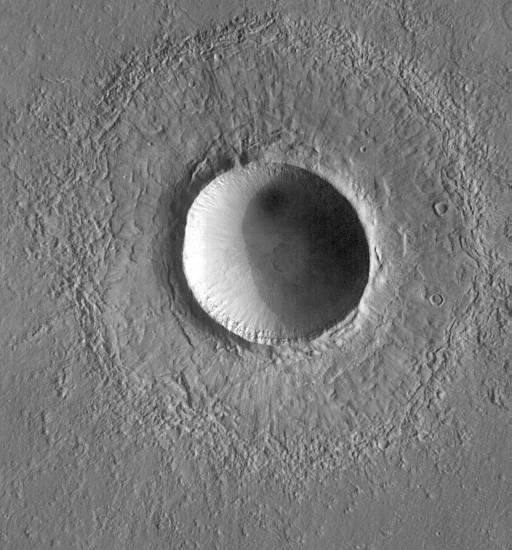
\includegraphics[width=0.2\textwidth]{images/Gre13_01.jpg} &
	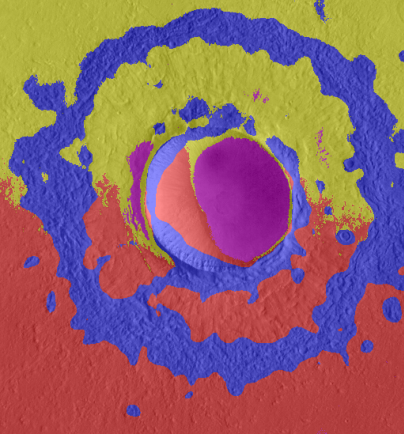
\includegraphics[width=0.2\textwidth]{images/gen/GEN_filterbanks_Gre13_01_TSUGF.png} &
	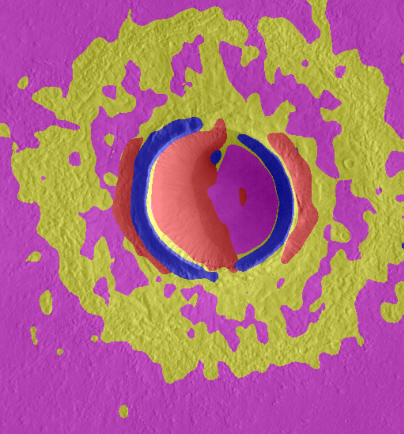
\includegraphics[width=0.2\textwidth]{images/gen/GEN_filterbanks_Gre13_01_LM.png} &
	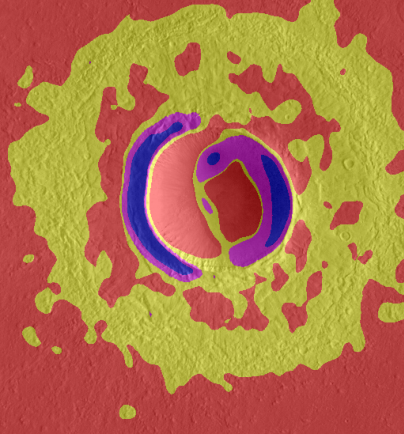
\includegraphics[width=0.2\textwidth]{images/gen/GEN_filterbanks_Gre13_01_S.png} &
	\includegraphics[width=0.2\textwidth]{images/gen/GEN_filterbanks_Gre13_01_MR.png} \\
	
	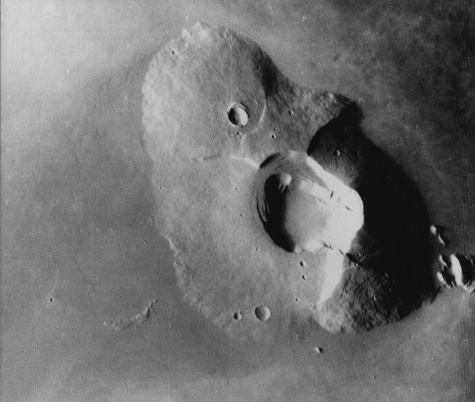
\includegraphics[width=0.2\textwidth]{images/Gre13_02.jpg} &
	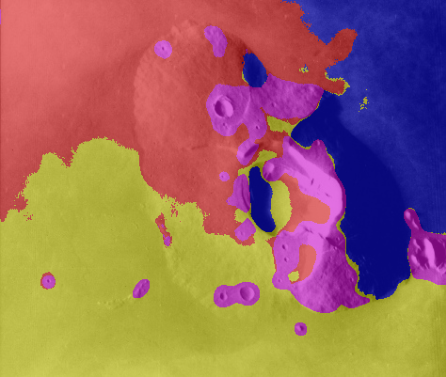
\includegraphics[width=0.2\textwidth]{images/gen/GEN_filterbanks_Gre13_02_TSUGF.png} &
	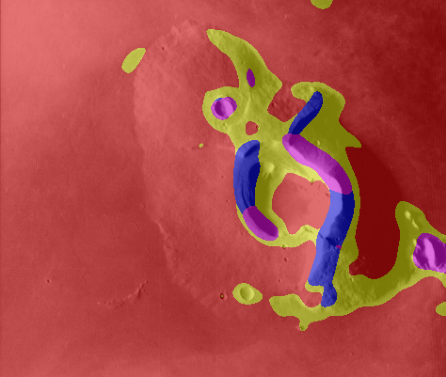
\includegraphics[width=0.2\textwidth]{images/gen/GEN_filterbanks_Gre13_02_LM.png} &
	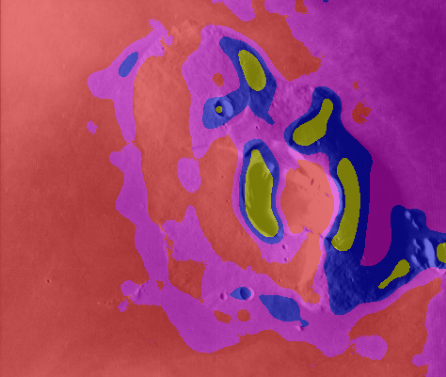
\includegraphics[width=0.2\textwidth]{images/gen/GEN_filterbanks_Gre13_02_S.png} &
	\includegraphics[width=0.2\textwidth]{images/gen/GEN_filterbanks_Gre13_02_MR.png} \\
	
	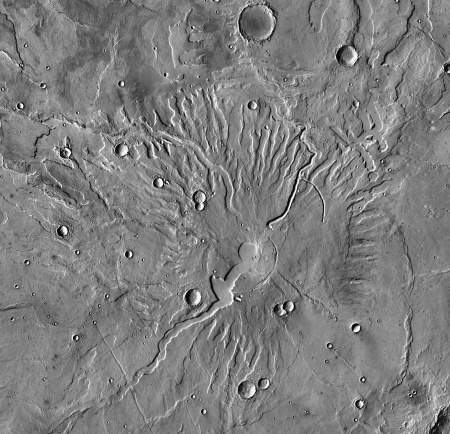
\includegraphics[width=0.2\textwidth]{images/Gre13_03.jpg} &
	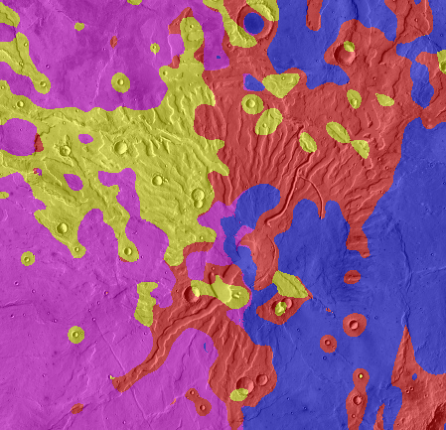
\includegraphics[width=0.2\textwidth]{images/gen/GEN_filterbanks_Gre13_03_TSUGF.png} &
	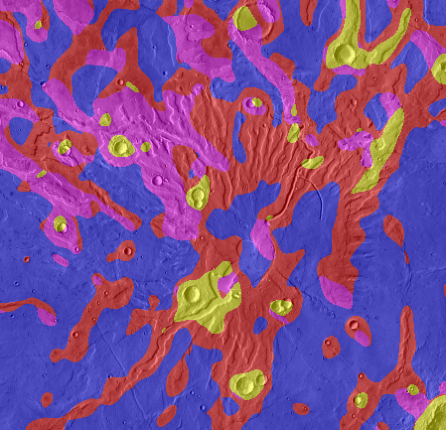
\includegraphics[width=0.2\textwidth]{images/gen/GEN_filterbanks_Gre13_03_LM.png} &
	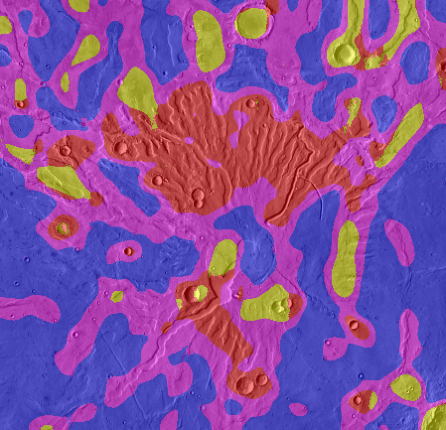
\includegraphics[width=0.2\textwidth]{images/gen/GEN_filterbanks_Gre13_03_S.png} &
	\includegraphics[width=0.2\textwidth]{images/gen/GEN_filterbanks_Gre13_03_MR.png} \\
	
	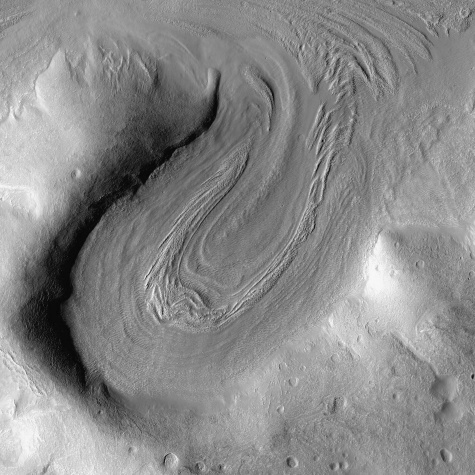
\includegraphics[width=0.2\textwidth]{images/Gre13_05.jpg} &
	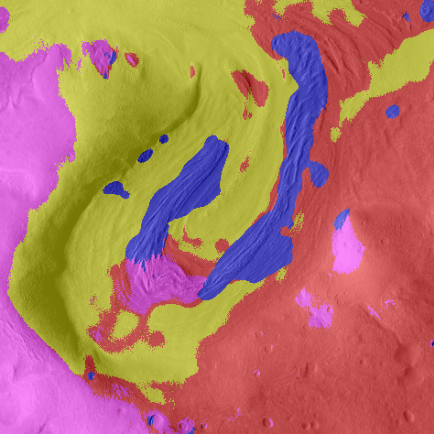
\includegraphics[width=0.2\textwidth]{images/gen/GEN_filterbanks_Gre13_05_TSUGF.png} &
	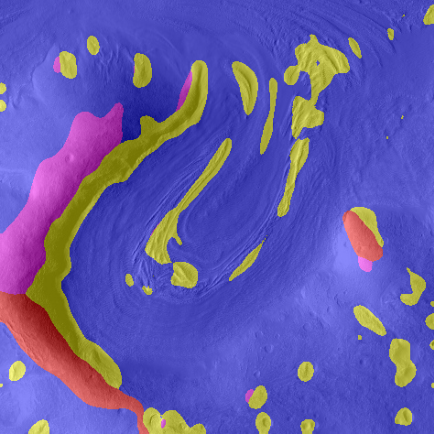
\includegraphics[width=0.2\textwidth]{images/gen/GEN_filterbanks_Gre13_05_LM.png} &
	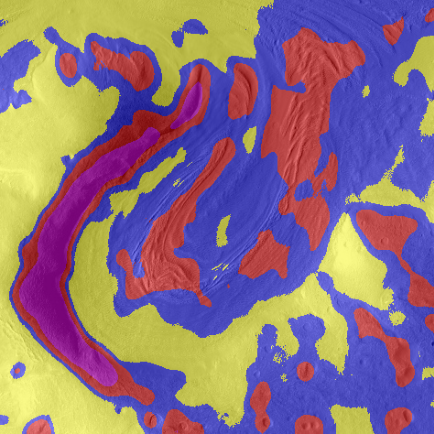
\includegraphics[width=0.2\textwidth]{images/gen/GEN_filterbanks_Gre13_05_S.png} &
	\includegraphics[width=0.2\textwidth]{images/gen/GEN_filterbanks_Gre13_05_MR.png} \\
	
	\hspace{1pt}\newline\centering Eingabe, aus \cite{greeley_13} &
	\hspace{1pt}\newline\centering Filterbank nach \cite{jain_91} &
	\hspace{1pt}\newline\centering LM-Filterbank \cite{leung_01} &
	\hspace{1pt}\newline\centering S-Filterbank \cite{schmid_01} &
	\hspace{1pt}\newline\centering MR-Filterbank \cite{visgeo} \\
\end{tabular}
\caption{Vergleich verschiedener Filterbänke auf Bildern der Marsoberfläche (Krater, Vulkan, Vulkan mit strahlenförmigen Merkmalen, Gletscher). Die Farben der jeweiligen Cluster wurden zufällig gewählt und sagen nichts über deren Inhalt aus. Alle Bilder wurden in vier Cluster eingeteilt.}
\label{fig:filterbank_comparision}
\end{figure}

\subsection{Größe der Filter}
\label{ssec:filtersize}

Neben der Auswahl einer geeigneten Filterbank lassen sich in dieser noch die einzelnen Gewichtungen anpassen: So könnten \zB die Gewichtung der Koordinaten der Pixel zueinander oder die Relevanz von ähnlichen Farbwerten modifiziert werden. Außerdem ist die Größe der einzelnen Filter in den jeweiligen Filterbänken auch Variabel und muss dementsprechend an die Dimensionen des jeweiligen Eingabebildes angepasst werden. Da alle Filterbänke (bis auf die nach \cite{jain_91}) jeweils gleiche Filter in unterschiedlichen Größen enthalten, muss nur ein Gesamtwert angepasst werden, statt der Größe jeder einzelnen Skalierung. Es wird nun versucht, die Ergebnisse der Maximum Response-Filterbank zu verbessern, da diese in vorherigen Versuchen die besten Ergebnisse erzielt hat.

Von dieser Stelle an müssen Marsaufnahmen genutzt werden, bei denen die Auflösung bekannt ist, somit scheiden die bis hierhin genutzten Aufnahmen aus \cite{greeley_13} leider aus. Stattdessen werden Ausschnitte aus der Aufnahme \texttt{P03\_002147\_1865\_XI\_06N208W} der Context Camera des Mars Reconnaissance Orbiters genutzt. Ein weiterer Vorteil der Nutzung dieser Bilder besteht daraus, dass die Clusteringalgorithmen nun an realitätsnähreren Daten getestet werden können, statt an isolierten Aufnahmen einzelner Besonderheiten der Oberfläche. Die Ergebnisse sind in \figurename~\ref{fig:filterbank_sizes} zu sehen. Als Startwert wurde ein Skalierungsfaktor $s=1$ betrachtet, angewandt auf die vorgestellten, quadratischen Filter mit einer originalen Kantenlänge von \SI{49}{\pixel}. Dieser wurde nach oben und unten hin in Schritten von $\Delta s=0.25$ verändert, und mit der skalierten MR-Filterbank ein neues Clustering der vier Ausschnitte erstellt. Die Eingabebilder sind quadratisch und besitzen eine Seitenlänge von \SI{650}{\pixel} bei einer Auflösung von \SI{6,17}{\meter\per\pixel}. Jedes der Eingabebilder wurde erneut in vier Bereiche eingeteilt, die Farben sind zur Veranschaulichung zufällig gewählt.

\paragraph{Skalierungsfaktor $s=0,25$}

Auf der ersten Aufnahme ist, vergleichbar mit den Beispielaufnahmen aus dem letzten Abschnitt, ein runder Krater zentriert zu sehen. Die geringe Skalierung mit dem Faktor $s=0.25$ führt dazu, dass die jeweiligen Filter zu klein sind, um die Strukturen der Oberfläche zu erkennen, somit sieht diese Aufnahme aus, als wäre nur anhand ihrer Helligkeitswerten geclustert worden. Das gleiche gilt auch für die zweite und vierte Aufnahme.

Die dritte Aufnahme stellt eine relativ ebenmäßige Fläche in einem Umfeld von gröberer Oberfläche dar. Dort scheint es, als gäbe es nicht genug Kontrast um nach den Helligkeitswerten zu clustern, der Algorithmus erstellt eine Filterung anhand der X- und Y-Koordinaten. Bei allen Aufnahmen werden nur zwei wirkliche Cluster erstellt, die letzten zwei Cluster die erstellt werden sollten bestehen nur aus jeweils wenigen Pixeln.

Dieser Skalierungsfaktor produziert keine brauchbaren Ergebnisse.

\paragraph{Skalierungsfaktor $s=0,50$}

Wie zu erwarten führt die genutzte, kleinere Skalierung mit $s=0,50$ der Filterbank zu vielen kleineren Clustern, in diesem Fall deutlich erkennbar anhand der gelb markierten Flächen. Obwohl es auf den ersten Blick scheint, als würden die Kraterränder erkannt werden, wird durch die Filterbank bei dieser Skalierung nur die dunkleren Bereiche, in diesem Fall die Schatten, die die erhöhten Kraterränder werfen, erkannt. Auf dieser Aufnahme führt dies zwar zu einer vergleichsweise guten Approxmimation der Krater, sobald anderweitige Schatten hinzukommen, wird diese Skalierung allerdings keine geeigneten Ergebnisse produzieren.

Das selbe Phänomen tritt auch bei der zweiten Aufnahme auf, auch dort wird stark anhand der Helligkeitswerte geclustert, erkennbar an den Kraterrändern. Bei diesem Bild wird allerdings auch trotz der kleineren Skalierung das raue Gebiet, welches sich horizontal durch das Bild erstreckt, in ein (violett gefärbtes) Cluster eingeteilt. Auch hier werden dunklerere Bereiche (wie die Kraterränder) in separate (gelb gefärbte) Cluster eingeteilt.

Auf der dritten Aufnahme wird bei der genutzten Skalierung die feinere Fläche größtenteils als ein (gelb gefärbtes) Cluster dargestellt, separat dazu sind in rot die Übergänge zwischen den Regionen gekennzeichnet. Die gröberen Flächen in den äußeren Bereichen werden nicht zuverlässig in das selbe Cluster eingeordnet.

Die letzte Testaufnahme, bestehend aus zwei Hügeln \bzw Bergen, stellt durch die über- und unterbelichteten Flächen an den Hängen eine der größten Herausforderungen für den Clusteringalgorithmus dar. An diesen Stellen ist der Kontrast des Bildes sehr gering, sodass kaum noch Texturen erkannt werden, anhand derer geclustert werden könnte. Wie zu erwarten werden die dunklen Flächen in ein einzelnes (violettes) Cluster kombiniert. Kleine Hügelketten hingegen werden zuverlässig in zusammengehörige Cluster eingeteilt, welches auf diesen Aufnahmen blau markiert ist. Die beleuchteten Seiten der Hügel werden bei dieser Skalierung leider nicht von der allgemeinen Marsoberfläche unterschieden.

Dieser Skalierungsfaktor führt zu vergleichsweise guten Clusteringergebnissen.

\paragraph{Skalierungsfaktor $s=0,75$}

Dieser Skalierungsfaktor führt beim Clustering des ersten Bildes zu Ergebnisse, welche vergleichbar mit denen des Faktors $s=0,5$ sind. Die Ränder der Krater werden allerdings in helle und dunkle Regionen eingeteilt, die Cluster im äußeren Bereich sind größer und gröber.

Auf der zweiten Aufnahme wird die horizontale rauere Region sehr gut in ein eigenes Cluster eingeteilt, selbiges gilt für die Kraterränder. Auf dieser Aufnahme erscheint der Skalierungsfaktor $s=0,75$ optimal.

Die dritte Aufnahme unterscheidet sich bis auf die gröberen, größeren Cluster in den äußeren Bereichen nicht wesentlich von der vorherigen Skalierung.

Bei der letzten Aufnahme führt die größere Skalierung zu einem uniformen Clusterings des beleuchteten Berghangs, er wird als eine große Fläche erkannt. Die dunkle Seite hingegen wird in zwei Cluster unterteilt: Die eigentliche dunkle Seite des Berges, und die Stellen, welche zu unterbelichtet sind, um aus ihnen eine Textur zu erkennen.

Insgesamt scheint sich dieser Skalierungsfaktor auch zum textutbasierten Clustering zu eignen.

\paragraph{Skalierungsfaktor $s=1.00$}

Während bei diesem Skalierungsfaktor auf der ersten Aufnahme der größere, mittigere Krater relativ gut durch ein rotes kreisförmiges Cluster gekennzeichnet wird, wird der kleinere Krater nicht zuverlässig erkannt. Bei diesem gehen die Cluster in umlegende Gebiete über, als wäre dieser Krater nur eine etwas rauere Oberflächenstruktur.

Bei der zweiten Aufnahme wird wie zuvor der Krater erfolgreich separat in ein Cluster eingeteilt, die Begrenzungen der gröberen Struktur, welche sich durch das Bild zieht, geht allerdings verloren. Diese Region wird leider im rechten Teil des Bildes sehr weitläufig erkannt.

In dem dritten Testbild werden die gröberen Hügelketten am Rand des helleren Bereiches zwar erkannt (gelb markiert), und die Übergangsstellen zwischen zwei Regionen werden in ein rotes Cluster zusammengefügt,  alle anderen Regionen sind allerdings nicht voneinander getrennt worden.

Das letzte Bild wird bei dieser Skalierung fast identisch zu der Skalierung mit $s=0,75$ geclustert.

Zusammengefasst ist diese Skalierung schon zu grob um so gute Ergbenisse wie die vorherigen zu erreichen.

\paragraph{Skalierungsfaktor $s=1.25$ und $s=1.50$}

Da diese beiden Skalierungsfaktoren zu fast identischen Clusterverteilungen führen, werden sie in einen Abschnitt zusammengefasst.

Bei diesen Skalierungen werden im oberen, glätteren Bereich der ersten Aufnahme die vereinzelten Krater wie gewollt erkannt, sie versagt allerdings im unteren, gröberen Bereich, wo sie nur ein großes Cluster erstellen. Der Krater wird nur anhand von starken Helligkeitsdifferenzen erkannt, welche in der gesamten Ausgabe violett bei $s=1,25$, \bzw blau bei $s=1,5$ markiert wurden. 

Selbiges gilt im Bezug auf die starken Helligkeitsdifferenzen bei der weiten Aufnahme.

Bei der dritten Aufnahme wird von beiden Skalierungsfaktoren kein brauchbares Ergebnis produziert, man kann höchstens erahnen, dass die jeweils blau gefärbten Regionen besonders kontrastarme, also glatte Flächen darstellen.

Beim Clusteringergebnis der letzten Aufnahme unterschieden sich die beiden Skalierungsfaktoren erstmals: Bei $s=1,25$ gleicht das Ergebnis dem des vorherigen Clusterings: Kleinere Bergregionen und rauere Oberflächenstrukturen werden getrennt voneinander Erkannt, Flächen mit weniger oder (aufgrund von Unterbelichtung) keiner werden auch in ein großes Cluster hinzugefügt. Der Faktor $s=1,5$ scheint selbst bei diesem Bild zu groß zu sein, bis auf die Hügelketten mit starker Helligkeitsdifferenz wird die Aufnahme nur anhand ihrer Helligkeitswerte geclustert.

Diese Faktoren sind also zu groß um brauchbare Ergebnisse zu produzieren.

\begin{figure}[h!]
	\setlength\tabcolsep{1pt}
	\def\arraystretch{0.5}
	\begin{tabular}{p{0.14\textwidth}p{0.14\textwidth}p{0.14\textwidth}p{0.14\textwidth}p{0.14\textwidth}p{0.14\textwidth}p{0.14\textwidth}}
		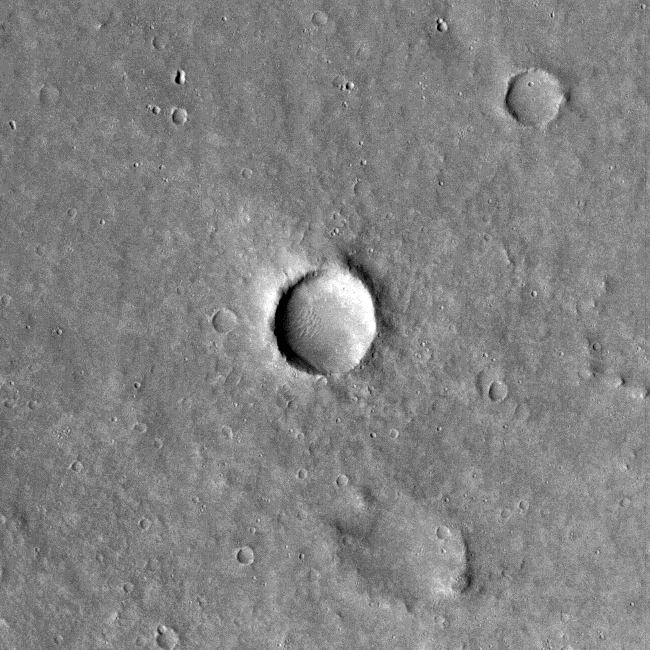
\includegraphics[width=0.14\textwidth]{images/p03_01.png} &
		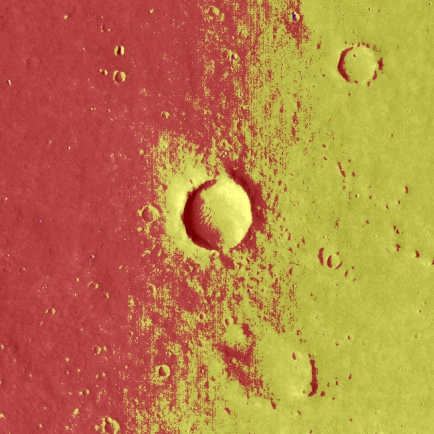
\includegraphics[width=0.14\textwidth]{images/gen/GEN_filterbanks_p03_01_MR_0.25.png} &
		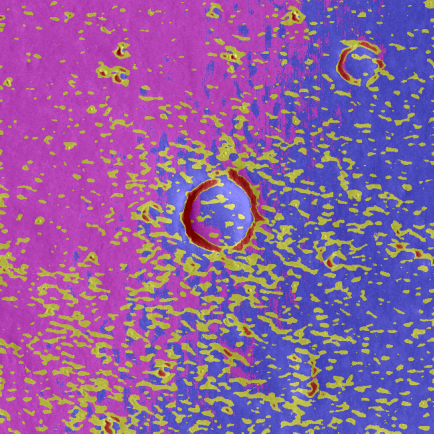
\includegraphics[width=0.14\textwidth]{images/gen/GEN_filterbanks_p03_01_MR_0.5.png} &
		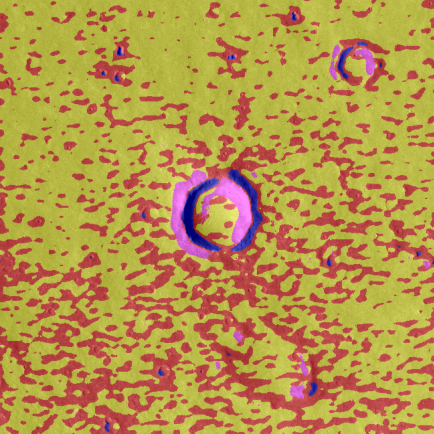
\includegraphics[width=0.14\textwidth]{images/gen/GEN_filterbanks_p03_01_MR_0.75.png} &
		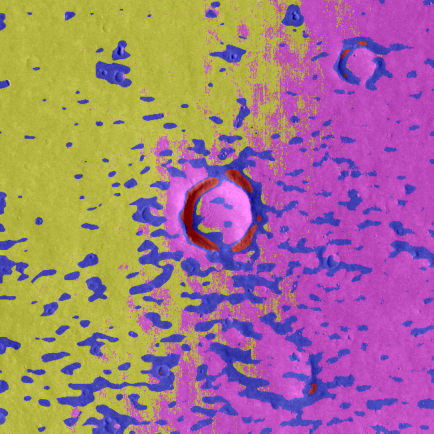
\includegraphics[width=0.14\textwidth]{images/gen/GEN_filterbanks_p03_01_MR_1.0.png} &
		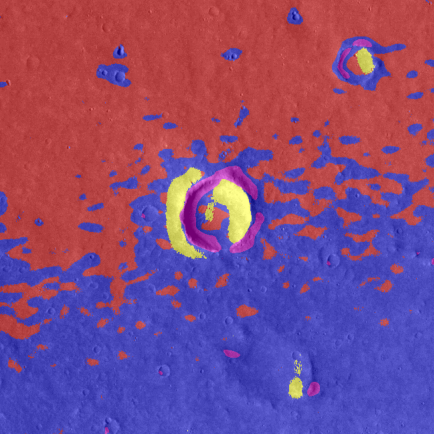
\includegraphics[width=0.14\textwidth]{images/gen/GEN_filterbanks_p03_01_MR_1.25.png} &
		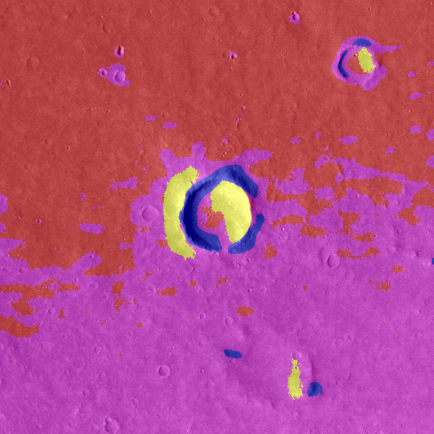
\includegraphics[width=0.14\textwidth]{images/gen/GEN_filterbanks_p03_01_MR_1.5.png} \\
		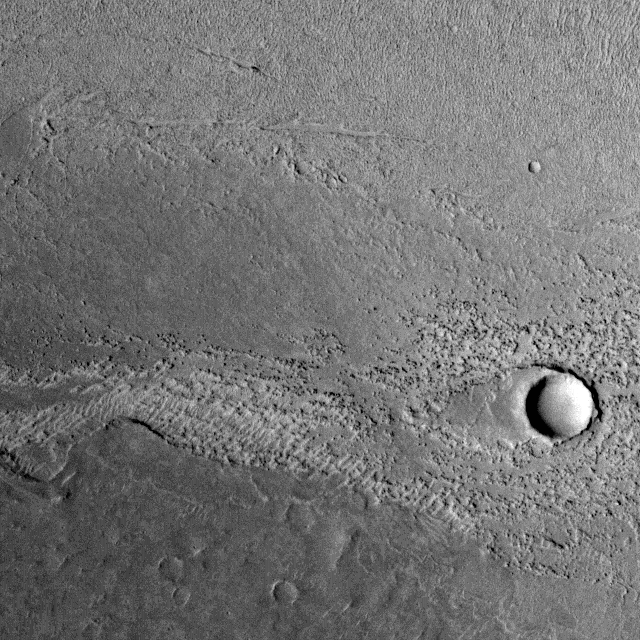
\includegraphics[width=0.14\textwidth]{images/p03_02.png} &
		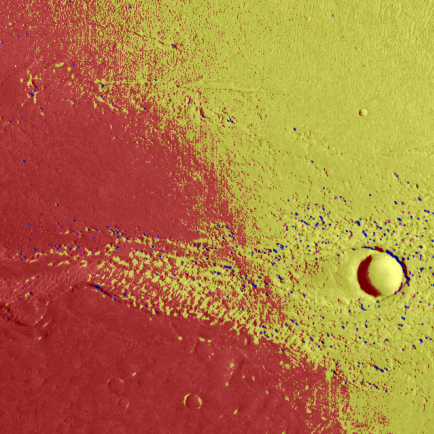
\includegraphics[width=0.14\textwidth]{images/gen/GEN_filterbanks_p03_02_MR_0.25.png} &
		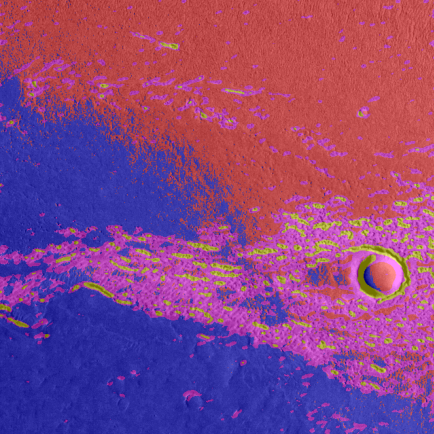
\includegraphics[width=0.14\textwidth]{images/gen/GEN_filterbanks_p03_02_MR_0.5.png} &
		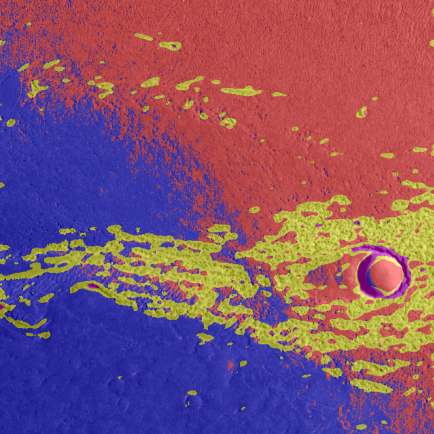
\includegraphics[width=0.14\textwidth]{images/gen/GEN_filterbanks_p03_02_MR_0.75.png} &
		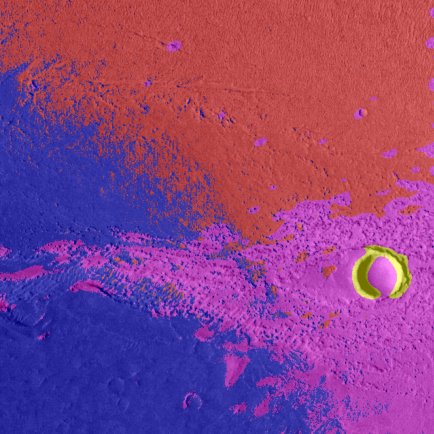
\includegraphics[width=0.14\textwidth]{images/gen/GEN_filterbanks_p03_02_MR_1.0.png} &
		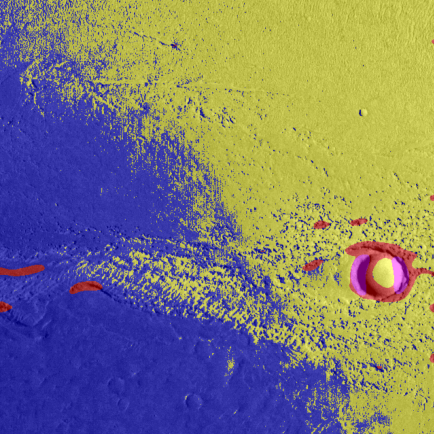
\includegraphics[width=0.14\textwidth]{images/gen/GEN_filterbanks_p03_02_MR_1.25.png} &
		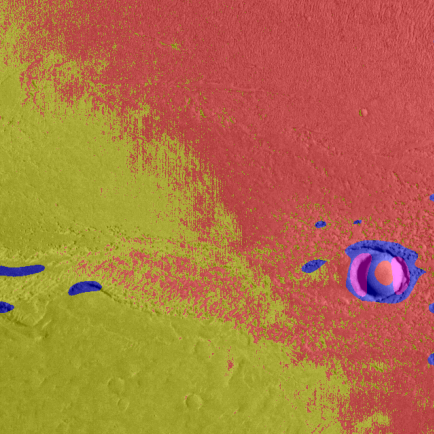
\includegraphics[width=0.14\textwidth]{images/gen/GEN_filterbanks_p03_02_MR_1.5.png} \\
		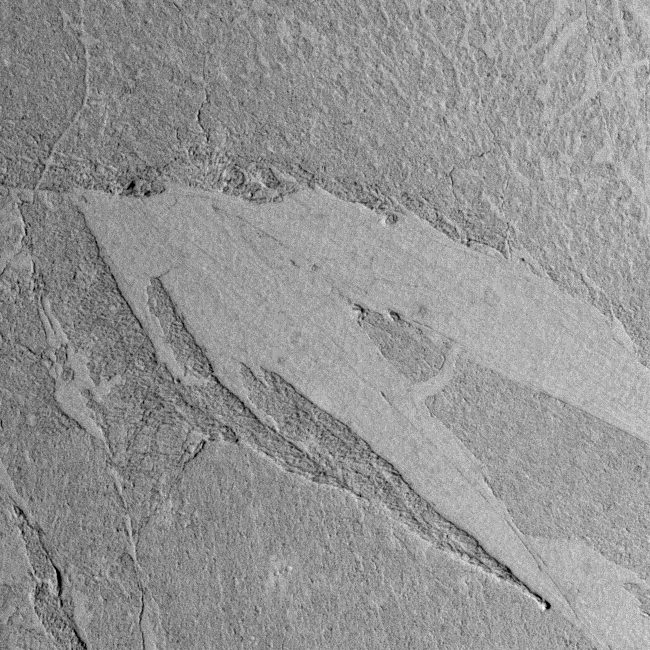
\includegraphics[width=0.14\textwidth]{images/p03_03.png} &
		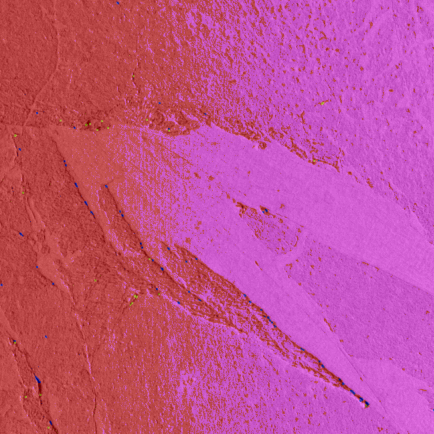
\includegraphics[width=0.14\textwidth]{images/gen/GEN_filterbanks_p03_03_MR_0.25.png} &
		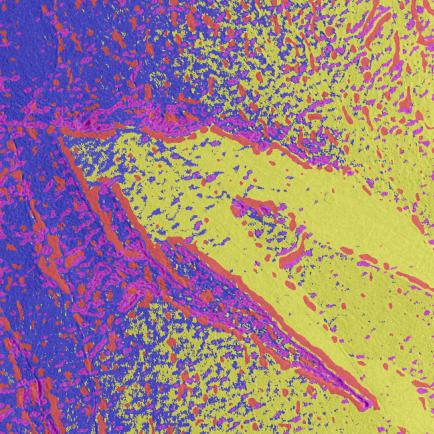
\includegraphics[width=0.14\textwidth]{images/gen/GEN_filterbanks_p03_03_MR_0.5.png} &
		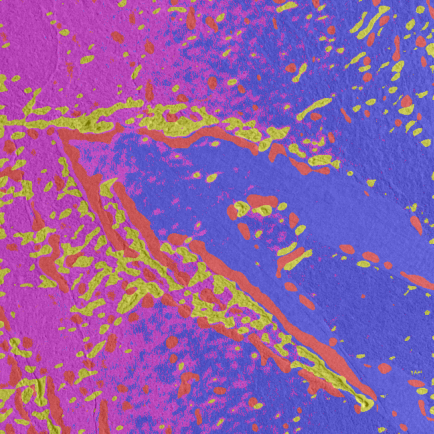
\includegraphics[width=0.14\textwidth]{images/gen/GEN_filterbanks_p03_03_MR_0.75.png} &
		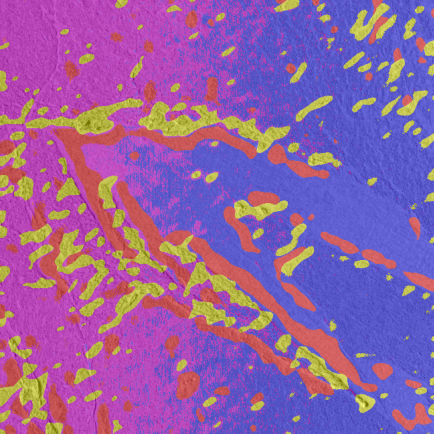
\includegraphics[width=0.14\textwidth]{images/gen/GEN_filterbanks_p03_03_MR_1.0.png} &
		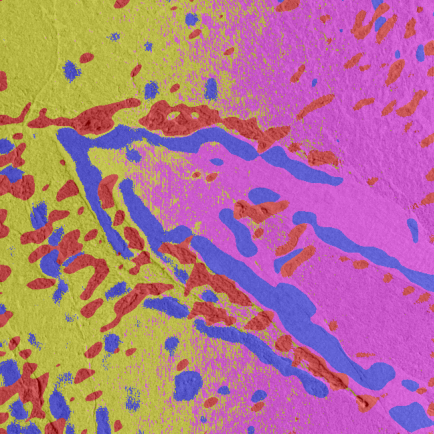
\includegraphics[width=0.14\textwidth]{images/gen/GEN_filterbanks_p03_03_MR_1.25.png} &
		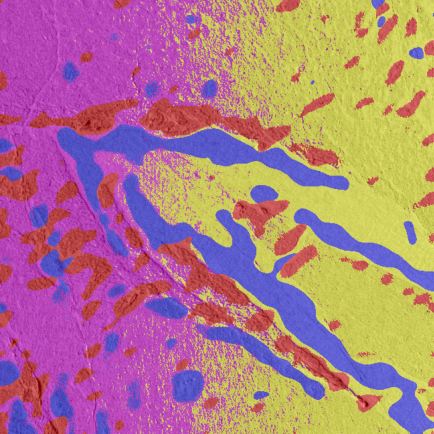
\includegraphics[width=0.14\textwidth]{images/gen/GEN_filterbanks_p03_03_MR_1.5.png} \\
		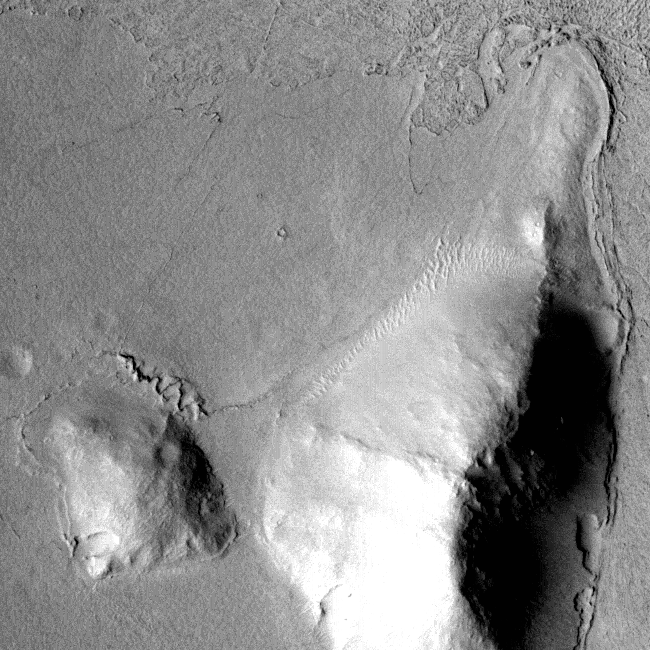
\includegraphics[width=0.14\textwidth]{images/p03_04.png} &
		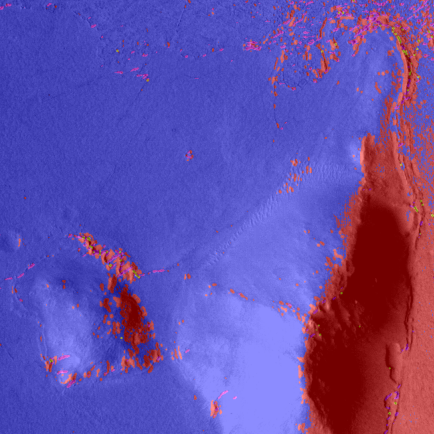
\includegraphics[width=0.14\textwidth]{images/gen/GEN_filterbanks_p03_04_MR_0.25.png} &
		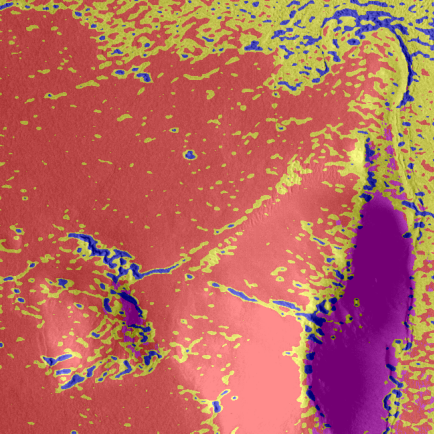
\includegraphics[width=0.14\textwidth]{images/gen/GEN_filterbanks_p03_04_MR_0.5.png} &
		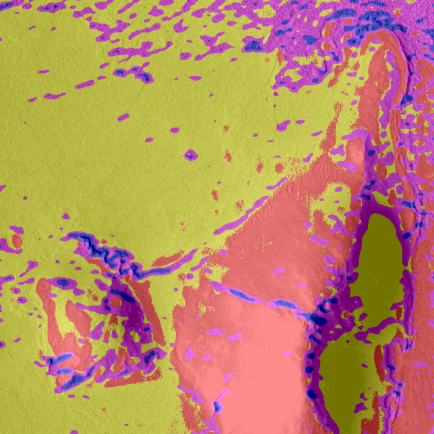
\includegraphics[width=0.14\textwidth]{images/gen/GEN_filterbanks_p03_04_MR_0.75.png} &
		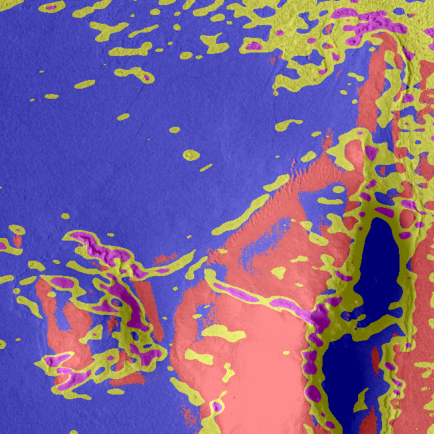
\includegraphics[width=0.14\textwidth]{images/gen/GEN_filterbanks_p03_04_MR_1.0.png} &
		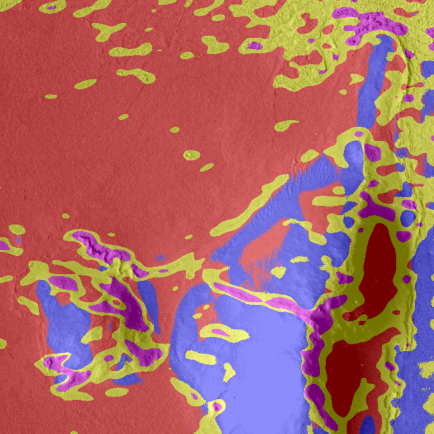
\includegraphics[width=0.14\textwidth]{images/gen/GEN_filterbanks_p03_04_MR_1.25.png} &
		\includegraphics[width=0.14\textwidth]{images/gen/GEN_filterbanks_p03_04_MR_1.5.png} \\
		
		\hspace{2pt}\newline\centering Eingabe & 
		\hspace{2pt}\newline\centering $s=0,25$ &
		\hspace{2pt}\newline\centering $s=0,50$ &
		\hspace{2pt}\newline\centering $s=0,75$ &
		\hspace{2pt}\newline\centering $s=1,00$ &
		\hspace{2pt}\newline\centering $s=1,25$ &
		\hspace{2pt}\newline\centering $s=1,50$
	\end{tabular}
	\caption{Vergleich verschiedener Skalierungen der MR-Filterbank auf Bildern der Marsoberfläche. Die Farben der jeweilgen Cluster wurden zufällig gewählt und sagen nichts über deren Inhalt aus. Alle Bilder wurden in vier Cluster eingeteilt.}
	\label{fig:filterbank_sizes}
\end{figure}

Aus diesen Ergebnissen lässt sich schlussfolgern, dass ein Skalierungsfaktor von $s=0,5$ bei diesen Eingabedaten die besten Ergebnisse liefert.

\subsection{Gewichtungen der Parameter}
\label{ssec:filterweight}

Da in dem Prozess des Clusterings alle Optimierungen aus Unterabschnitt~\ref{ssec:tsugf} miteingeschlossen sind, beinhaltet dies, dass der Datenwürfel, den k-Means verarbeitet, sowohl die Koordinaten, als auch die Farbwerte der Eingabedatei beinhaltet. Nun stellt sich die Frage, wie stark diese jeweils gewichtet werden sollten, um ein akzeptables Ergebnis zu erhalten. Aus diesem Grund sind in den Abbildungen~\ref{fig:filterbank_weights_pos} und \ref{fig:filterbank_weights_col} die Ergebnisse des Clusterings mit unterschiedlichen Werten für die jeweiligen Gewichtungen zu sehen. Die Skalierung der Filter beträgt $s=0,5$, da im vorherigen Unterabschnitt festgestellt wurde, dass dieser Wert relativ gute Ergebnisse liefert.

\paragraph{Gewichtung der Koordinaten}
Das Hinzufügen der X- und Y-Koordinaten zu dem Datenwürfel ist ursprünglich aus dem Grund geschehen, dass ein gegebener räumlicher Bezug zwischen unterschiedlichen Pixeln beim Clustering berücksichtigt werden kann (\vgl Unterabschnitt~\ref{ssec:tsugf}; \cite{jain_91}). Aus den Clusteringergebnissen in \figurename~\ref{fig:filterbank_weights_pos} allerdings lässt sich erkennen, dass dieser räumliche Bezug in diesem Anwendungsfall nicht außerordentlich hilfreich ist: Bei einer Gewichtung von $w_p\geq1,33$ lässt sich eindeutig erkennen, dass der allgemeine Bodenbereich auf allen Aufnahmen zu stark Anhand seiner Positionen eingeteilt wird, es entstehen Cluster in den Ecken der Aufnahmen, welche sich ins Zentrum erstrecken. Unter diesem starken Einfluss nimmt zusätzlich die relative Wichtigkeit der ähnlichen Textur ab.

Wird nun ein geringerer Wert für $w_p$ betrachtet, so erkennt man für Werte mit $w_p\leq0.66$ keinen Starken Unterschied bei wechselnden Gewichtungen. Dies ist insbesondere bei $w_p=0$ signifikant, da dort der räumliche Bezug der einzelnen Pixel zueinander bei der Berechnung des Clusterings zwar komplett ignoriert wird, das eigentliche Ergebnis sich --~bis auf etwas kleinere Cluster in den merkmalsarmen Bereichen~-- aber kaum verändert. Dies lässt sich darauf zurückführen, dass das Hinzufügen des räumlichen Bezuges ursprünglich den Grund hatte, dass auf \enquote{normalen} Fotografien die vorkommenden Cluster meistens nur ein einziges mal an einem räumlich begrenzten Ort vorhanden sind, so sind \zB bei der Aufnahme aus \figurename~\ref{fig:tsugf_optim} aus Unterabschnitt~\ref{ssec:tsugf} die kleineren Korallen im linken Hintergrund nur an dieser Stelle vorhanden und ließen sich durch ein weit ausgedehntes Cluster zusammenfassen. Bei den aktuell genutzten Aufnahmen hingegen ist dies nicht der Fall, eine auftretende Oberflächenstruktur, wie \zB ein Krater kann an verschieden Stellen ohne räumlichen Bezug zueinander auftreten.
Die Nutzung der Positionwerte hat allerdings einen Vorteil: Sie sorgt dafür die Clustergrößen nicht zu klein und fragmentiert werden zu lassen, indem sie eine Relation mit benachbarten Pixeln erzeugt, welche der k-Means Algorithmus berücksichtigt.

Aus diesem Grund macht es Sinn, die Koordinatenbeträge der Pixel relativ gering zu gewichten, um dafür zu sorgen, dass das texturbasierte Clustering möglicht positionsinvariant operiert, aber auch nicht so gering, dass viele fragmentierte Cluster entstehen. Anhand von \figurename~\ref{fig:filterbank_weights_pos} ist erkennbar, dass ein Wert von  $w_p=0,66$ sich in diesem Fall sehr gut eignet, ein Clusterergebnis zu erstellen.

\begin{figure}[h!]
	\setlength\tabcolsep{1pt}
	\def\arraystretch{0.5}
	\begin{tabular}{p{0.14\textwidth}p{0.14\textwidth}p{0.14\textwidth}p{0.14\textwidth}p{0.14\textwidth}p{0.14\textwidth}p{0.14\textwidth}}
		\includegraphics[width=0.14\textwidth]{images/p03_01.png} &
		\includegraphics[width=0.14\textwidth]{images/gen/GEN_filterbanks_p03_01_MR_pos_0.png} &
		\includegraphics[width=0.14\textwidth]{images/gen/GEN_filterbanks_p03_01_MR_pos_0.33.png} &
		\includegraphics[width=0.14\textwidth]{images/gen/GEN_filterbanks_p03_01_MR_pos_0.66.png} &
		\includegraphics[width=0.14\textwidth]{images/gen/GEN_filterbanks_p03_01_MR_pos_1.0.png} &
		\includegraphics[width=0.14\textwidth]{images/gen/GEN_filterbanks_p03_01_MR_pos_1.33.png} &
		\includegraphics[width=0.14\textwidth]{images/gen/GEN_filterbanks_p03_01_MR_pos_1.66.png} \\
		\includegraphics[width=0.14\textwidth]{images/p03_02.png} &
		\includegraphics[width=0.14\textwidth]{images/gen/GEN_filterbanks_p03_02_MR_pos_0.png} &
		\includegraphics[width=0.14\textwidth]{images/gen/GEN_filterbanks_p03_02_MR_pos_0.33.png} &
		\includegraphics[width=0.14\textwidth]{images/gen/GEN_filterbanks_p03_02_MR_pos_0.66.png} &
		\includegraphics[width=0.14\textwidth]{images/gen/GEN_filterbanks_p03_02_MR_pos_1.0.png} &
		\includegraphics[width=0.14\textwidth]{images/gen/GEN_filterbanks_p03_02_MR_pos_1.33.png} &
		\includegraphics[width=0.14\textwidth]{images/gen/GEN_filterbanks_p03_02_MR_pos_1.66.png} \\
		\includegraphics[width=0.14\textwidth]{images/p03_03.png} &
		\includegraphics[width=0.14\textwidth]{images/gen/GEN_filterbanks_p03_03_MR_pos_0.png} &
		\includegraphics[width=0.14\textwidth]{images/gen/GEN_filterbanks_p03_03_MR_pos_0.33.png} &
		\includegraphics[width=0.14\textwidth]{images/gen/GEN_filterbanks_p03_03_MR_pos_0.66.png} &
		\includegraphics[width=0.14\textwidth]{images/gen/GEN_filterbanks_p03_03_MR_pos_1.0.png} &
		\includegraphics[width=0.14\textwidth]{images/gen/GEN_filterbanks_p03_03_MR_pos_1.33.png} &
		\includegraphics[width=0.14\textwidth]{images/gen/GEN_filterbanks_p03_03_MR_pos_1.66.png} \\
		\includegraphics[width=0.14\textwidth]{images/p03_04.png} &
		\includegraphics[width=0.14\textwidth]{images/gen/GEN_filterbanks_p03_04_MR_pos_0.png} &
		\includegraphics[width=0.14\textwidth]{images/gen/GEN_filterbanks_p03_04_MR_pos_0.33.png} &
		\includegraphics[width=0.14\textwidth]{images/gen/GEN_filterbanks_p03_04_MR_pos_0.66.png} &
		\includegraphics[width=0.14\textwidth]{images/gen/GEN_filterbanks_p03_04_MR_pos_1.0.png} &
		\includegraphics[width=0.14\textwidth]{images/gen/GEN_filterbanks_p03_04_MR_pos_1.33.png} &
		\includegraphics[width=0.14\textwidth]{images/gen/GEN_filterbanks_p03_04_MR_pos_1.66.png} \\
		
		\hspace{2pt}\newline\centering Eingabe & 
		\hspace{2pt}\newline\centering $w_p=0,00$ &
		\hspace{2pt}\newline\centering $w_p=0,33$ &
		\hspace{2pt}\newline\centering $w_p=0,66$ &
		\hspace{2pt}\newline\centering $w_p=1,00$ &
		\hspace{2pt}\newline\centering $w_p=1,33$ &
		\hspace{2pt}\newline\centering $w_p=1,66$
	\end{tabular}
	\caption{Vergleich verschiedener Gewichtungen der Koordinaten beim Clustering der jeweiligen Eingabedateien. Die Farben der jeweilgen Cluster wurden zufällig gewählt und sagen nichts über deren Inhalt aus. Alle Bilder wurden in vier Cluster eingeteilt.}
	\label{fig:filterbank_weights_pos}
\end{figure}

\paragraph{Gewichtungen der Farb-/Helligkeitswerte}
Die hier folgenden Clusteringergebnisse wurden mit einem Skalierungsfaktor von $s=0,5$ und einer Gewichtung von $w_p=0,66$ für die Positionswerte erstellt.

In der originalen Ausarbeitung des texturbasierten Clusterings \cite{jain_91} werden nur zwei Ebenen für die jeweiligen X- und Y-Koordinaten hinzugefügt. Es steht also an dieser Stelle offen, ob das Hinzufügen der Farb- \bzw Helligkeitsdimension zum Datenwürfel zu besseren Ergebnissen führt. Dazu wurde der vorgestellte Algorithmus mit unterschiedlichen Werten für die Gewichtung der Helligkeitswerte $w_c$ auf den bekannten Beispielbildern ausgeführt. Die Ergebnisse dieses Experimentes sind in \figurename~\ref{fig:filterbank_weights_col} dargestellt.

Auf diesen Clusterings wird schnell ersichtlich, dass eine Veränderung der Gewichtung relativ geringe Auswirkungen hat. Eine stärkere Gewichtung von $w_c=1,66$ besitzt auf der vierten Aufnahme den wohl größten Einfluss, da dort anhand der Über- und Unterbelichtung die beiden Bergseiten getrennt voneinander erkannt werden. Obwohl diesese Phänomen hier gute Auswirkungen hat, ist es im allgemeinen ungewollt: Mit diesem starken Einfluss der Helligkeitswerte lernt das neuronale Netzwerk stärker mithilfe der Helligkeit statt über die Textur dieser Cluster zu lernen, was eines der größten Probleme beim Trainieren dieses Netzes ist.

Da sich durch die zusätzlichen Helligkeitswerte keine Verbesserungen der Clusteringergebnisse feststellen lassen wird dieser Schritt von nun an entfernt, es gilt also $w_c=0$.

\begin{figure}[h!]
	\setlength\tabcolsep{1pt}
	\def\arraystretch{0.5}
	\begin{tabular}{p{0.14\textwidth}p{0.14\textwidth}p{0.14\textwidth}p{0.14\textwidth}p{0.14\textwidth}p{0.14\textwidth}p{0.14\textwidth}}
		\includegraphics[width=0.14\textwidth]{images/p03_01.png} &
		\includegraphics[width=0.14\textwidth]{images/gen/GEN_filterbanks_p03_01_MR_col_0.png} &
		\includegraphics[width=0.14\textwidth]{images/gen/GEN_filterbanks_p03_01_MR_col_0.33.png} &
		\includegraphics[width=0.14\textwidth]{images/gen/GEN_filterbanks_p03_01_MR_col_0.66.png} &
		\includegraphics[width=0.14\textwidth]{images/gen/GEN_filterbanks_p03_01_MR_col_1.0.png} &
		\includegraphics[width=0.14\textwidth]{images/gen/GEN_filterbanks_p03_01_MR_col_1.33.png} &
		\includegraphics[width=0.14\textwidth]{images/gen/GEN_filterbanks_p03_01_MR_col_1.66.png} \\
		\includegraphics[width=0.14\textwidth]{images/p03_02.png} &
		\includegraphics[width=0.14\textwidth]{images/gen/GEN_filterbanks_p03_02_MR_col_0.png} &
		\includegraphics[width=0.14\textwidth]{images/gen/GEN_filterbanks_p03_02_MR_col_0.33.png} &
		\includegraphics[width=0.14\textwidth]{images/gen/GEN_filterbanks_p03_02_MR_col_0.66.png} &
		\includegraphics[width=0.14\textwidth]{images/gen/GEN_filterbanks_p03_02_MR_col_1.0.png} &
		\includegraphics[width=0.14\textwidth]{images/gen/GEN_filterbanks_p03_02_MR_col_1.33.png} &
		\includegraphics[width=0.14\textwidth]{images/gen/GEN_filterbanks_p03_02_MR_col_1.66.png} \\
		\includegraphics[width=0.14\textwidth]{images/p03_03.png} &
		\includegraphics[width=0.14\textwidth]{images/gen/GEN_filterbanks_p03_03_MR_col_0.png} &
		\includegraphics[width=0.14\textwidth]{images/gen/GEN_filterbanks_p03_03_MR_col_0.33.png} &
		\includegraphics[width=0.14\textwidth]{images/gen/GEN_filterbanks_p03_03_MR_col_0.66.png} &
		\includegraphics[width=0.14\textwidth]{images/gen/GEN_filterbanks_p03_03_MR_col_1.0.png} &
		\includegraphics[width=0.14\textwidth]{images/gen/GEN_filterbanks_p03_03_MR_col_1.33.png} &
		\includegraphics[width=0.14\textwidth]{images/gen/GEN_filterbanks_p03_03_MR_col_1.66.png} \\
		\includegraphics[width=0.14\textwidth]{images/p03_04.png} &
		\includegraphics[width=0.14\textwidth]{images/gen/GEN_filterbanks_p03_04_MR_col_0.png} &
		\includegraphics[width=0.14\textwidth]{images/gen/GEN_filterbanks_p03_04_MR_col_0.33.png} &
		\includegraphics[width=0.14\textwidth]{images/gen/GEN_filterbanks_p03_04_MR_col_0.66.png} &
		\includegraphics[width=0.14\textwidth]{images/gen/GEN_filterbanks_p03_04_MR_col_1.0.png} &
		\includegraphics[width=0.14\textwidth]{images/gen/GEN_filterbanks_p03_04_MR_col_1.33.png} &
		\includegraphics[width=0.14\textwidth]{images/gen/GEN_filterbanks_p03_04_MR_col_1.66.png} \\
		
		\hspace{2pt}\newline\centering Eingabe & 
		\hspace{2pt}\newline\centering $w_c=0,00$ &
		\hspace{2pt}\newline\centering $w_c=0,33$ &
		\hspace{2pt}\newline\centering $w_c=0,66$ &
		\hspace{2pt}\newline\centering $w_c=1,00$ &
		\hspace{2pt}\newline\centering $w_c=1,33$ &
		\hspace{2pt}\newline\centering $w_c=1,66$
	\end{tabular}
	\caption{Vergleich verschiedener Gewichtungen der Farb- \bzw Helligkeitswerte beim Clustering der jeweiligen Eingabedateien. Die Farben der jeweilgen Cluster wurden zufällig gewählt und sagen nichts über deren Inhalt aus. Alle Bilder wurden in vier Cluster eingeteilt.}
	\label{fig:filterbank_weights_col}
\end{figure}

\section{Netzwerkarchitektur}
\label{sec:networkarch}

Die Netzwerkarchitektur im originalen Paper stellt ein relativ einfaches Netzwerk zur Objekterkennung oder Bildsegmentierung dar: Es durchläuft iterativ eine Reihe mit je einer Convolutional Layer, gefolgt von einer Batch Normalization. Im Folgenden wird geprüft, ob eine Modifikation dieser Architektur in diesem domänenspezifischen Anwendungsfall zu Verbesserungen der Ergebnisse führen kann.

\subsection{Aktivierungsfunktionen}
\label{ssec:arch_activation}

\subsection{Pooling Layer}
\label{ssec:arch_pooling}

\subsection{Fully Connected Layers}
\label{ssec:arch_fully}

\section{Hyperparameter}
\label{sec:hyperparameter}

\section{Abbruchkriterium}
\label{sec:stoppingcriteria}

\section{Preprocessing}
\label{sec:preprocessing}

\section{Anpassungen für mehrfarbige Fotografien}
\label{sec:referenceimages}